

\chapter{ Capítulo introductorio}

\begin{chapquote}{Javier, \textit{Todos los días}}
`` Me cago en Dios''
\end{chapquote}

\section{La visión como herramienta}

\subsection{La visión en el ser humano}
El ser humano es capaz de interactuar con el mundo que le rodea de diversas maneras ya sean creativas, constructivas o banales. Esto se puede conseguir mediante los sentidos; Tacto, gusto, oído, olfato y por último pero no menos importante la visión. Este último sentido nos permite recoger gran cantidad de información de nuestro entorno, procesarla y actuar en consecuencia. Es entonces el ojo humano una herramienta de gran valor y elevada precisión que poco tiene que envidiar al órgano análogo en el resto de especies en todo el reino animal. 

Lejos de realizar un estudio anatómico del sentido de la vista en el ser humano, se disponen a continuación ciertas características de interés que permiten apreciar toda su potencia.

Una de las primeras cuestiones que se vienen a la mente cuando se habla de la "simple vista" es su resolución, es decir, cuál es la mínima distancia que es capaz de distinguir. Se puede estudiar mediante la resolución angular que para el ser humano se encuentra entorno a 1' o 2' o l que es lo mismo un intervalo de 0,02º a 0,03º\cite{simple_vista}. Dicho de otra forma, un ojo humano sano y correctamente desarrollado puede distinguir objetos de entre 30cm y 60cm a 1km de distancia. Por ejemplo, una persona podría detectar dos balones de playa de un diámetro aproximado de 45cm hasta 1km de distancia.

%https://es.wikipedia.org/wiki/Simple_vista

El campo de visión es también un aspecto de gran importancia ya que determina la cantidad de información que los ojos pueden recibir en un instante dado. El "cono de visión" queda entorno a unos 130º en vertical y 160º en horizontal que equivale aproximadamente a una lente con longitud focal de 2mm\cite{angle_of_view}. Se entiende como distancia focal, en el ámbito de la fotografía, la distancia entre el punto en el que convergen los rayos de luz formando una imagen y el sensor digital del dispositivo. Esta medida se determina cuando la lente está enfocada al infinito.

En resumidas cuentas, a mayor distancia focal, más estrecho será el ángulo de visión y mayor la magnificación ocurriendo el efecto contrario según se reduce la distancia focal. Se muestra en la figura \ref{fig:focal_length} un esquema de lo explicado: 


\begin{figure}[!htb]
\centering
\minipage{0.7\textwidth}
  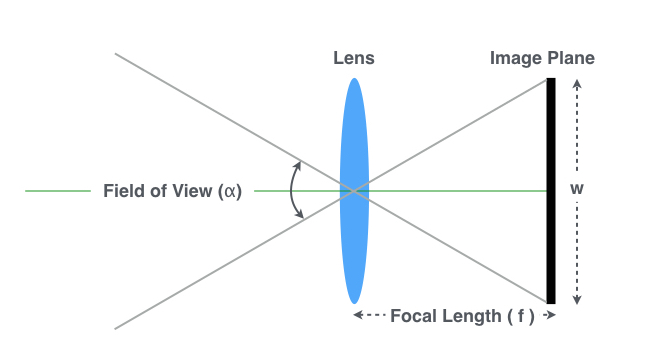
\includegraphics[width=\linewidth]{focal_length}
  \caption{Ángulo de visión en función de la distancia focal}\label{fig:focal_length}
\endminipage\hfill

\end{figure}

%https://en.wikipedia.org/wiki/Angle_of_view#Common_lens_angles_of_view


Por último, se considera la velocidad de enfoque o acomodación del ojo humano. Según un experimento llevado cabo por el MIT\cite{mit_experiment} (Massachussets Institute of Technology) el ojo humano es capaz de captar una imagen para su posterior procesamiento en tan solamente 13 milisegundos.

Este experimento consistía en  mostrar un conjunto de seis o doce imágenes y de entre las cuales se pedía a los participantes identificar "una pareja sonriente" o un entorno de campo. 
Para llegar al resultado actual, el equipo del MIT comenzó proyectando imágenes a una velocidad de exposición de 80 milisegundos. Posteriormente se redujo poco a poco este tiempo solamente para las imágenes que había que identificar pasando a 53 milisegundos, luego de 40 a 27, y finalmente se llegaron a los 13 milisegundos. Posteriores reducciones del tiempo de exposición hacían imposible identificar las imágenes.

%http://www.sophimania.pe/ciencia/cerebro-y-neurociencias/estudio-revela-que-el-ojo-humano-capta-una-imagen-en-13-milisegundos/
%http://news.mit.edu/2014/in-the-blink-of-an-eye-0116

Se ha planteado entonces una situación en la que hay un pequeño problema, un instrumento de gran precisión y prolongada durabilidad embarcado en un ser vivo falible y errático. No sólo esto sino que nunca se llega a dominar por completo el manejo de éste órgano así como su uso en conjunto a las demás partes del cuerpo y siempre todo ello limitado por la velocidad de respuesta que puede proporcionar el sistema nervioso.
Bienes sabido que los deportistas de alta competición deben poseer una capacidad de reacción casi inmediata a diferentes tipos de estímulos como lo son sonoros o visuales, es decir, una bocina o un semáforo, por ejemplo. 

Existen dos tipos de tiempos de reacción\cite{tiempo_reaccion}; simple y complejo. El primero hace referencia al tiempo que transcurre desde la recepción de un estímulo anticipado o ya conocido hasta la reacción, mientras que el segundo se diferencia en el tipo de estímulo ya que en este caso es desconocido o se considera un imprevisto. Resulta obvio que el tiempo de reacción simple es menor que el complejo porque la respuesta está decidida de antemano. 

Además, se ha de considerar que la respuesta a estímulos sonoros es más rápida que a los estímulos visuales. Esto se debe a que los receptores auditivos se estimulan mecánicamente (vibración de los huesos del oído debido a una onda sonora) mientras que los visuales lo hacen de forma química.

Habiendo visto estas consideraciones y tomando como referencia los datos de Mateyev 1977 y los estudios de Cometti se disponen en la tabla  datos relevantes sobre tiempos de reacción en atletas y no atletas.

ALTO NIVEL      SONORA  0,05 – 010
LUMINOSA  0,10 – 0,20

NO ATLETAS      SONORA  0,15 – 0,25 y más
LUMINOSA  0,20 – 0,35 Y MÁS

Es decir, en el mejor de los casos y para un atleta profesional, se tarda un quinto de segundo en reaccionar a un estímulo predefinido y por tanto, sabiendo la reacción que hay que llevar a cabo tal y como puede ser poner en movimiento un vehículo al ver la luz verde en un semáforo.
%https://www.fuerzaycontrol.com/la-velocidad-de-reaccion-el-tiempo-de-reaccion-simple-complejo-la-anticipacion/

Aunque la vista en conjunto con el sistema nervioso nos permiten llevar a cabo, en ocasiones, tareas impensables como se pueden ver en deportes de alta competición o en la prestidigitación, por ejemplo, podemos manejar una herramienta todavía más potente, la inteligencia. Entre las muchas definiciones del mencionado concepto se puede ver la siguiente:

"Capacidad de tomar decisiones para resolver problemas"


Esta idea está inevitablemente ligada al término "tecnología" que se puede introducir como:

"La aplicación de conocimientos científicos para la resolución de problemas mediante el diseño y creación de bienes y servicios" 

junto a su etimología, pues se trata de una palabra de origen griego 
%τεχνολογία 
formada por 
%τέχνη 
(arte, técnica u oficio) y 
%λογία 
(el estudio de algo) es fácil apreciar que la evolución y desarrollo del ser humano junto a su inteligencia durante toda su historia han venido ligadas a un progreso tecnológico\cite{historia_tecnologia} incesante, vivo y capaz de abrirse paso incluso en las épocas más oscuras de la historia de la humanidad como se ve en la figura \ref{fig:history_technology} 

\begin{figure}[!htb]
\centering
\minipage{0.7\textwidth}
  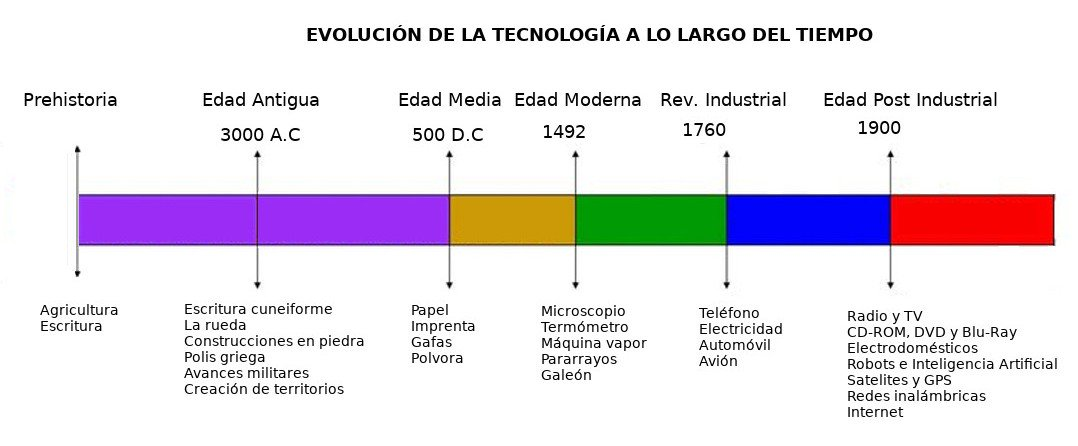
\includegraphics[width=\linewidth]{history_technology}
  \caption{Línea temporal de los pregresos tecnológicos más importantes de la hiistoria}\label{fig:history_technology}
\endminipage\hfill
\end{figure}
%https://tecnomagazine.net/2018/04/30/historia-de-la-tecnologia/

Es concretamente en el siglo XX cuando aparecen inventos revolucionarios, que cambian el curso de la historia marcando un definido punto de inflexión en la misma. Véanse por ejemplo la radio, el transistor, o internet. Uno de los impactos más notables es el incremento de la población mundial debido al progreso tecnológico entre otros factores. Se unifican ambos conceptos en la figura \ref{fig:technology_population}

\begin{figure}[!htb]
\centering
\minipage{0.65\textwidth}
  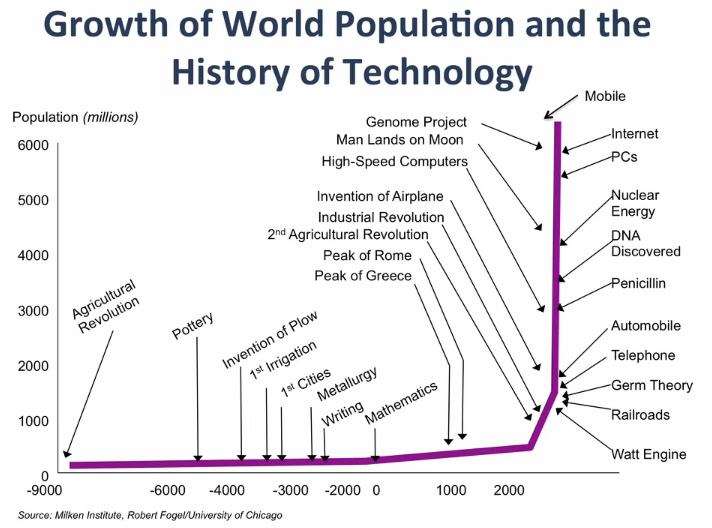
\includegraphics[width=\linewidth]{technology_population}
  \caption{Evolución conjunta de la población mundial y tecnología}\label{fig:technology_population}
\endminipage\hfill
\end{figure}

\subsection{Exportando la capacidad de visión}

Una vez descritas brevemente la potencia, capacidad y posibilidades que aporta la visión en el ser humano junto a su capacidad de resolver problemas mediante la tecnología, se puede ir más allá, subir un nivel y dotar a entes ajenos al hombre de la habilidad de obtener y procesar información visual. Este concepto existe desde finales de la década de los sesenta y puede introducirse como visión artificial o visión por computador\cite{vision_artificial}:
\\
“Disciplina científica que incluye métodos para adquirir, procesar, analizar y comprender las imágenes del mundo real con el fin de producir información numérica o simbólica para que puedan ser tratados por un computador”
\\
Esta forma de trabajar con información visual es posible debido a la puesta en conjunto de diferentes campos como la geometría, física o estadística y demás herramientas que se explicarán más adelante.
%https://es.wikipedia.org/wiki/Visi%C3%B3n_artificial#Detecci%C3%B3n_de_objetos

Bien es cierto que se plantea un problema ya que la forma en que el ojo humano percibe el mundo no es la misma en la que lo hace una máquina pues se pueden establecer sus diferencias como las mismas que hay entre una señal analógica y otra digital, respectivamente.
\\
Véase en primer lugar la mencionada diferencia respecto a las señales:

\begin{itemize}
\item Señal analógica
\\
Se trata de la representación de una magnitud física tal y como se percibe del entorno o se genera con algún instrumento y puede verse como una función matemática continua.
La mayoría de las señales que se perciben son analógicas como ejemplo la intensidad de corriente eléctrica, la temperatura, el sonido, presión y energía.
De este modo existen señales analógicas periódicas (caracterizadas por amplitud y frecuencia) no periódicas (toman cualquier valor independientemente del tiempo). Un ejemplo de señal analógica periódica\cite{señal_analogica} se ve en la figura \ref{fig:analog_signal}

\begin{figure}[!htb]
\centering
\minipage{0.65\textwidth}
  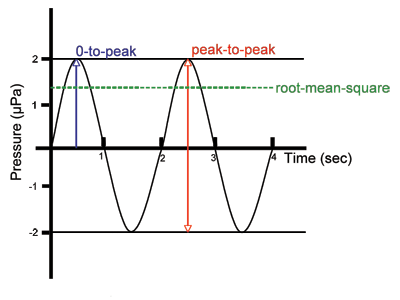
\includegraphics[width=\linewidth]{analog_signal}
  \caption{Señal analógica que representa una onda sonora bajo el mar. Se muestran tres formas de caracterizar su intensidad: Valor de cero a pico, valor de pico a pico y raíz cuadrada del valor medio.}\label{fig:analog_signal}
  
\endminipage\hfill
\end{figure}
%https://dosits.org/science/advanced-topics/introduction-to-signal-levels/

\item Señal digital
\\
Existe una extendida confusión en lo referente a la diferencia entre señal digital y señal discretizada. Se puede partir de una señal analógica senoidal y entonces llegar a una señal discretizada tomando valores equidistantes en el tiempo como se muestra en la figura \ref{fig:analogica_digitalizada}:
\begin{figure}[!htb]
\centering
\minipage{0.65\textwidth}
  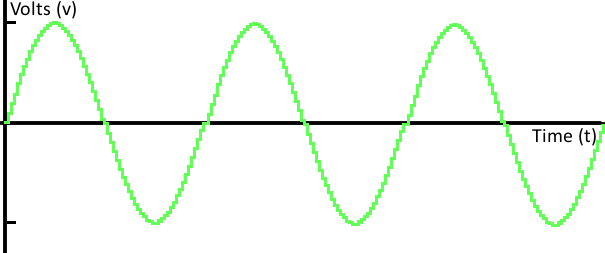
\includegraphics[width=\linewidth]{analogica_digitalizada}
  \caption{Señal analógica discretizada. En cada instante de tiempo se tiene un valor perteneciente a un conjunto fijo.}\label{fig:analogica_digitalizada}
\endminipage\hfill
\end{figure}
%https://learn.sparkfun.com/tutorials/analog-vs-digital/digital-signals

Para obtener una señal digital, se codifican cada uno de los valores discretos de la señal representada anteriormente. De este modo se tiene un número finito de valores pertenecientes a un conjunto y no intervalos.

Se puede mostrar en la figura \ref{fig:adc} el funcionamiento básico de un convertidor Analógico/digital para comprender la diferencia entre estos dos conceptos.

\begin{figure}[!htb]
\centering
\minipage{0.65\textwidth}
  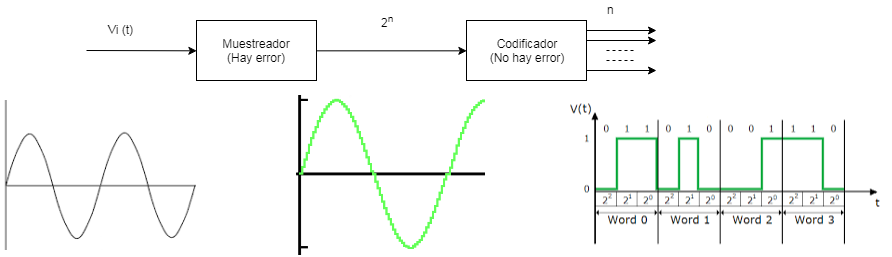
\includegraphics[width=\linewidth]{adc}
  \caption{Convertidor analógico-digital. La señal digital resultante forma palabras con  bits, es decir, se tienen en total $2^3=8$  valores diferentes y únicos}\label{fig:adc}
\endminipage\hfill
\end{figure}

Llevando esta idea al campo de los sistemas digitales, tal y como puede ser un ordenador, se llega al uso de la lógica de dos estados o binaria en la cual existen los estados alto H o 1 y bajo L o 0 en el caso de lógica positiva y H o 0 junto a L o 1 para la lógica negativa.
Un ejemplo de señal digital para la lógica de dos estados:

\begin{figure}[!htb]
\centering
\minipage{0.65\textwidth}
  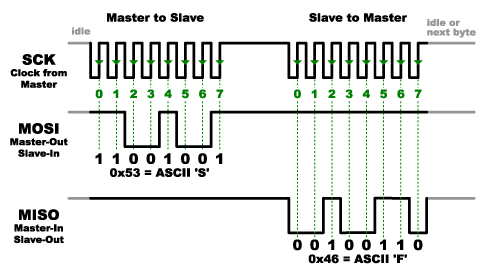
\includegraphics[width=\linewidth]{digital_signal}
  \caption{Ejemplo de comunicación maestro escalvo mediante señales digitales.}\label{fig:digital_signal}
\endminipage\hfill
\end{figure}

\end{itemize}

%https://difiere.com/la-diferencia-analogo-digital/

Volviendo al enfrentamiento entre el funcionamiento de la visión humana y artificial, se establece la comparación de ambas a continuación:

\begin{itemize}
\item Ojo humano
\\
Por una parte el ser humano recibe información visual tal y como se describiría en un mundo analógico,es decir, de forma continua.
\\
Sin entrar en demasiado detalle en el ámbito anatómico, la visión en el hombre se explica como la capacidad del ojo para detectar la luz y transformar la energía lumínica en señales eléctricas las cuales viajan al cerebro mediante el nervio óptico. Entre sus componentes principales se encuentran la córnea, la parte más externa del ojo, el cristalino, una lente ajustable según la distancia al objetivo así como un "diafragma" denominado pupila, cuyo diámetro está regulado por el iris, y la retina que se trata del tejido sensible a la luz. 

El funcionamiento del ojo se explica porque la luz es refractada por la córnea al atravesarla. Esta luz refractada pasa a través de la pupila y el cristalino y se proyecta sobre la retina, zona en la que unas células fotorreceptoras la transforman en impulsos nerviosos que se trasladan, a través del nervio óptico, al cerebro.

%https://steemit.com/science/@greenrun/the-human-eye-and-vision-a-fascinating-phenomenon

\begin{figure}[!htb]
\centering
\minipage{0.50\textwidth}
  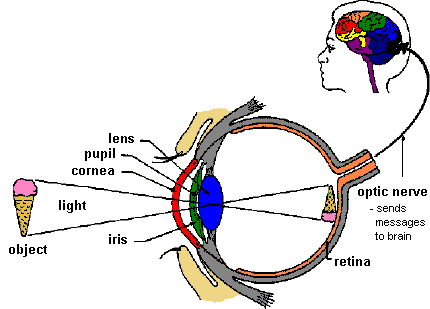
\includegraphics[width=\linewidth]{human_vision}
  \caption{Esquema del proceso de adquisición de información visual a través del ojo.}\label{fig:human_vision}
\endminipage\hfill
\end{figure}

Se ve claramente un tipo de señal analógica presente en el proceso, la luz, o mejor dicho la intensidad de la misma que pude representarse por la luminancia, es decir, candela por metro cuadrado.

%https://es.wikipedia.org/wiki/Intensidad_luminosa
%https://es.wikipedia.org/wiki/Ojo_humano#Examen_del_ojo

\item Sensor artificial
\\
No se puede aplicar de forma directa el concepto del funcionamiento del ojo humano en un sensor artificial ya que trabaja con información digitalizada. 

De este modo hace falta unos pasos intermedios antes de llegar a un resultado final Por lo tanto hay que utilizar una aproximación diferente para resolver el problema y es aquí donde entra el concepto de nube de puntos. 
\end{itemize}

\section{Concepto de nube de puntos} \label{section:nubes_ejemplo}

Una nube de puntos se puede definir como una estructura $P$ que representa un conjunto de puntos multidimensionales $p \subset R_{n}$. En el caso de una nube de puntos en tres dimensiones, es decir $n=3$, cada elemento o punto está representado como mínimo por sus coordenadas geométricas $X,Y, Z$ respecto a un sistema de referencia dado. Pero se puede añadir más datos todavía en forma de color, curvatura o información sobre la normal $\vec{n}$ a una superficie en un ámbito local de la misma.  


Por lo tanto una nube de puntos es un conjunto de puntos individuales sin relación alguna entre ellos, cuya
posición, color y otro tipo de características tienen definición, edición y representación muy simple por lo
que es realmente práctico y sencillo manejar una gran cantidad de ellos sin tener que preocuparse por
conceptos como escala, rotaciones y demás relaciones entre diferentes puntos de un mismo objeto, siempre y cuando se tome la consideración más básica de la idea de nube de puntos.

%https://www.3deling.com/whta-is-a-point-cloud/
%https://www.3deling.com/rgb-point-cloud/

Se puede derivar de este concepto una gran potencia y flexibilidad ya que si se tienen una cantidad
suficiente de puntos dispuestos correctamente se pueden representar todo tipo de superficies aunque en
realidad no se trate de un plano continuo, es decir, el cerebro es capaz de interpretar complejas formas a
partir de un tipo de información tan sencilla como las tres coordenadas espaciales.

Es más, se pueden llevar a cabo conversiones para relacionar el conjunto de puntos de la nube y crear
superficies reales en tres dimensiones. Este tipo de conversión se denomina también como reconstrucción de superficies, es decir, se parte de información puntual y se crea una superficie continua estimando qué
relación puede haber entre puntos cercanos. De esta forma, una nube de puntos puede transformarse a una
malla de polígonos o triángulos o incluso modelos CAD.

Las técnicas de reconstrucción de superficies son variadas y entre ellas se encuentran la triangulación de
delaunay, que construye una red de triángulos sobre los vértices de la nube de puntos.

Sobre la triangulación de delaunay, se debe cumplir la condición que toma el mismo nombre sobre la nube de puntos en la que se quiere reconstruir la superficie y la cual establece que:
\\
"la circunferencia circunscrita de un triángulo no debe contener ningún otro vértice de la triangulación en su interior, admitiéndose vértices situados sobre la circunferencia"
\\
En este contexto se entiende que por "vértice" se indica un punto de la nube de puntos.
Por lo tanto una red de triángulos es una triangulación de Delaunay si todos y cada uno de los triángulos que la forman cumplen la condición descrita que puede aplicarse tanto en espacios bidimensionales como tridimensionales.

La apreciación gráfica del mencionado concepto puede verse a continuación:
\begin{figure}[!htb]
\minipage{0.32\textwidth}
  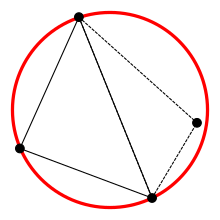
\includegraphics[width=\linewidth]{delaunay_mal}
  \caption{Vértice en el interior de una circunferencia circunscrita. No se cumple la condición de Delaunay}\label{fig:del_mal}
\endminipage\hfill
\minipage{0.32\textwidth}
  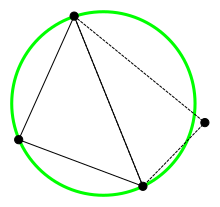
\includegraphics[width=\linewidth]{delaunay_bien}
  \caption{Vértice fuera de una circunferencia circunscrita. Se cumple la condición de Delaunay}\label{fig:del_bien}
\endminipage\hfill
\minipage{0.32\textwidth}
  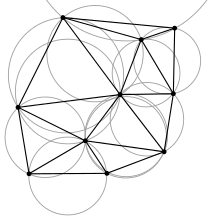
\includegraphics[width=\linewidth]{delaunay_bien_10pts}
	\caption{Triangulación de Delaunay aplicada a 10 puntos. Ninguna de las circunferencias circunscritas contiene vértices en su interior.}\label{fig:del_bien_10pts}
\endminipage
\end{figure}
El origen del nombre de la condición de Delauany se debe al matemático ruso Boris Nikolaevich Delone quien lo ideó en 1934 y tomó la forma francesa de su apellido, "Delaunay" como referencia a sus antecesores franceses.

%https://en.wikipedia.org/wiki/Point_cloud

Por otra parte, una peculiaridad o limitación respecto a las nubes de puntos tiene que ver con que la
información que representan es superficial, es decir, los puntos siempre pertenecen a la superficie del
objeto en cuestión ya que es el lugar donde la luz de los escáneres se llega, rebota y devuelve la
información correspondiente, proceso que se explica con más profundidad en apartados posteriores.

Otra desventaja inherente a las nubes de puntos es la interpretación de la información que contienen ya
que se ha explicado que está compuesta de un conjunto de objetos o puntos sin relación entre ellos. Es
aquí donde se requiere intervención del ser humano pues es su cerebro el que puede encontrar la similitud
entre una nube de puntos dada y el objeto o escenario que se supone que representa. Existe software capaz
de encontrar patrones y características para clasificar nubes de puntos pero nunca de forma
completamente fiable.

El concepto de nube de puntos es eminentemente simple así como versátil y de gran utilidad. Esto se puede apreciar con gran multitud de aplicaciones del concepto de nube de puntos en el mundo real y es que este progreso tecnológico es un gran paso adelante para refinar procesos ya existentes, desde producción a nivel industrial hasta establecer las bases de la navegación de cualquier robot o vehículo.

Se muestran a continuación varios ejemplos de diferentes características:

En primer lugar se tiene en la figura \ref{fig:bunny_simple} una sencilla nube de puntos que representa un conejo. Se ha tomado una captura desde uno de todos los posibles puntos de vista que ofrece una visión en 360º.
Un ejemplo algo más elaborado se recoge en la figura \ref{fig:wolf} en la que aparece una nube que representa un lobo. 
Otro ejemplo de mayor complejidad permite observar en la figura \ref{fig:botes} un escaneo frontal de tres botes de plástico. En este caso, es obvio que las zonas vacías justo detrás de los botes son aquellos lugares donde los rayos de luz emitidos por el sensor no pueden llegar ya que los propios botes los bloquean lo cual sirve para que su superficie quede capturada. Además, se ha incluido un campo de color para cada punto.


\begin{figure}[!htb]
\minipage{0.32\textwidth}
  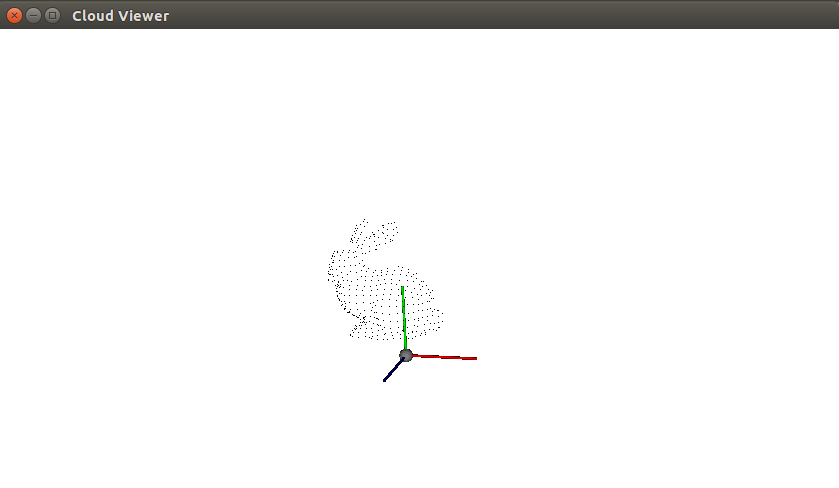
\includegraphics[width=\linewidth]{bunny_simple}
  \caption{Nube de puntos representando un conejo.
  Peso total de la nube: 10.6KB.
  Número total de puntos: 397.}\label{fig:bunny_simple}
\endminipage\hfill
\minipage{0.32\textwidth}
  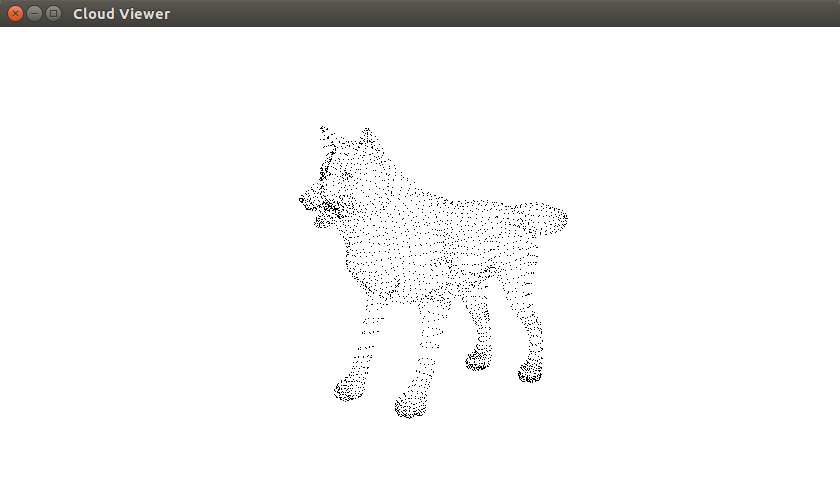
\includegraphics[width=\linewidth]{wolf}
  \caption{Nube de puntos representando un lobo.
  Peso total de la nube: 42.6KB.
  Número total de puntos: 3400.}\label{fig:wolf}
\endminipage\hfill
\minipage{0.32\textwidth}%
  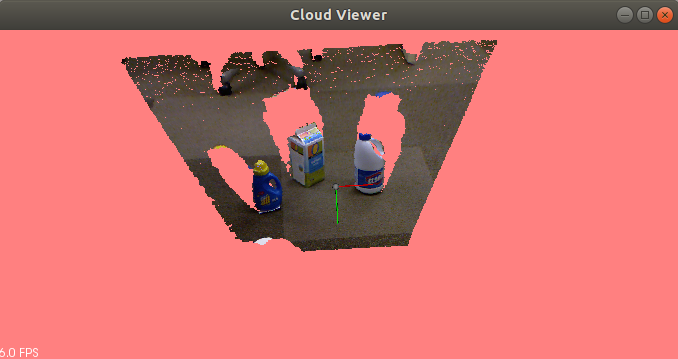
\includegraphics[width=\linewidth]{botes}
  \caption{Nube de puntos representando tres botes.
  Peso total de la nube: 2.43MB.
  Número total de puntos: 307200.}\label{fig:botes}
\endminipage
\end{figure}


%http://www.pointclouds.org/news/2013/01/07/point-cloud-data-sets/
%http://graphics.stanford.edu/data/3Dscanrep/
%http://kos.informatik.uni-osnabrueck.de/3Dscans/
%https://www.cc.gatech.edu/~turk/bunny/bunny.html

Una vez vistos ejemplos de nubes de puntos con la información suficiente para reconocer qué objeto representan sin más ayuda que la de los propios ojos, es momento de subir el nivel de complejidad para dar lugar a nubes de puntos como las que se muestran a continuación:

Se ha visto anteriormente una sencilla representación de un conejo con solamente 397 puntos. El nivel de detalle pude incrementarse a niveles del orden de decenas de miles de puntos tal y como es el caso de la figura \ref{fig:bunny} que representa un conejo de arcilla de 7.5 pulgadas de alto con unos 69451 triángulos ya que se ha llevado a cabo la reconstrucción de la superficie. Además, en la figura \ref{fig:bunny_colored} se aprecia el resultado si se añade información sobre color en cada punto.
Como consecuencia de añadir más información (más de 90 veces la cantidad de puntos y el color) se tiene en este caso un peso de 22MB con hasta 35947 puntos.
\begin{figure}[!htb]
\minipage{0.45\textwidth}
  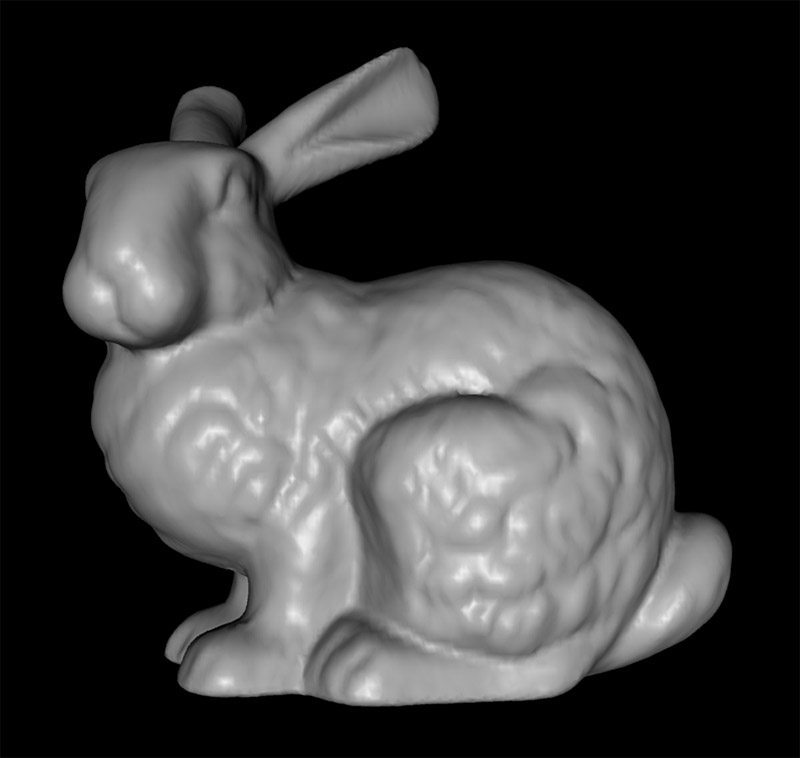
\includegraphics[width=\linewidth]{bunny}
  \caption{Nube de puntos con reconstrucción de superficie representando un conejo sin información de color.}\label{fig:bunny}
\endminipage\hfill
\minipage{0.45\textwidth}
  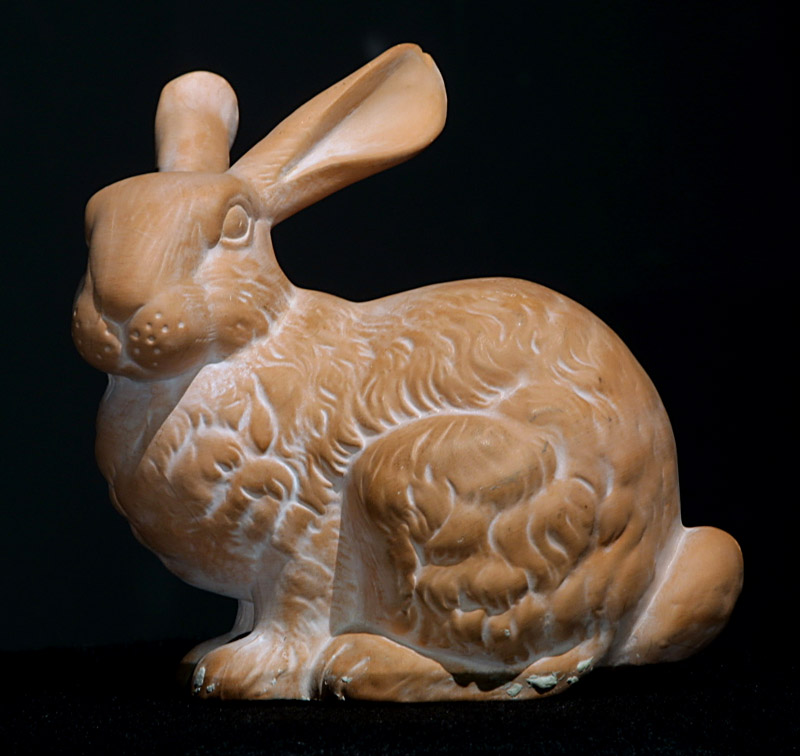
\includegraphics[width=\linewidth]{bunny_colored}
  \caption{Nube de puntos con reconstrucción de superficie representando un conejo con información de color.}\label{fig:bunny_colored}
\endminipage\hfill
\end{figure}
Esta nube de puntos proviene del departamento de computación gráfica de la universidad de Stanford e hicieron falta un total de 10 escaneos con el escaner Cyberware 3030 MS para llegar al resultado final. Para hacerse una idea del tipo de sensor utilizado, se tiene como dato relevante su precio de unos 10000 dólares (ebay) teniendo en cuenta además de que se trata de un sensor antiguo pues el escaneo se produjo en 1993.

%https://www.ebay.com/itm/Cyberware-Rapid-3D-Digitizer-Model-Shop-Color-3030-Scanner-3030RGB-MS-/372338340673?_ul=AR

Se pueden representar objetos más grandes y con mayor nivel de detalle tal y como se aprecia en la figura \ref{fig:dragon} que representa un dragón construido con madera y resina y con un tamaño de aproximadamente 20cm x 8cm x 9cm.

\begin{figure}
\centering
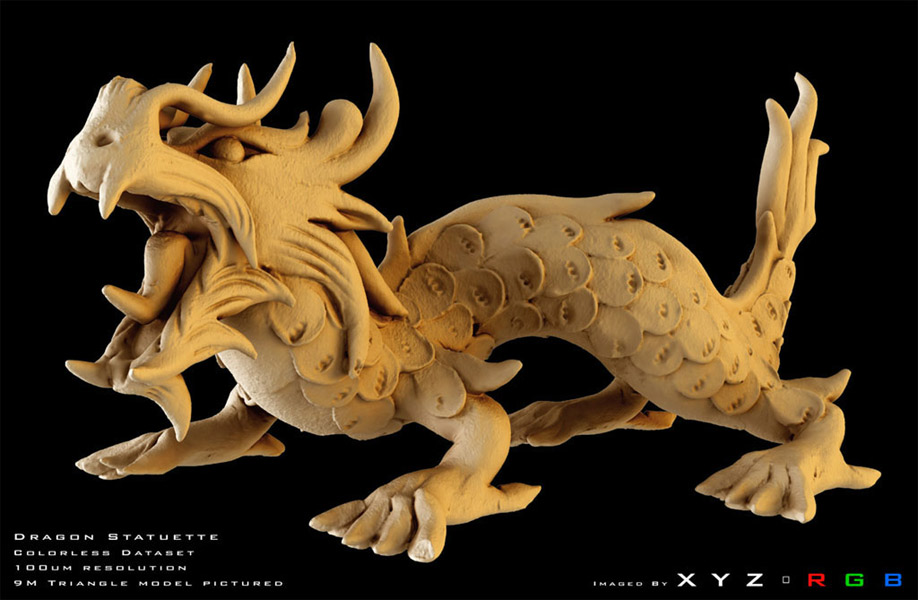
\includegraphics[scale=0.3]{dragon}
\caption{Nube de puntos con reconstrucción de superficie representando una figura de un dragón.}\label{fig:dragon}
\end{figure}

En este caso se han llevado a cabo 18 escaneos con una resolución de 100$\mu$m o lo que es lo mismo, la separación entre puntos es del orden de 0,1mm. Se dispone de un total de 3609455 puntos y 7218906 triángulos lo que implica un peso de 86MB para la nube reconstruida y descomprimida.
La nube de puntos se generó en el mismo laboratorio y con el mismo escaner que se ha mencionado en el caso anterior.

Otro objeto de elevada complejidad que ha sido escaneado en las mismas condiciones que el dragón y el conejo es el ángel Lucy. Un total de 47 escaneos dan lugar a un resultado final de 14027932 puntos y 28055742 triángulos y para este caso un peso de 508MB tomando la nube de puntos reconstruida y descomprimida.

\begin{figure}
\centering
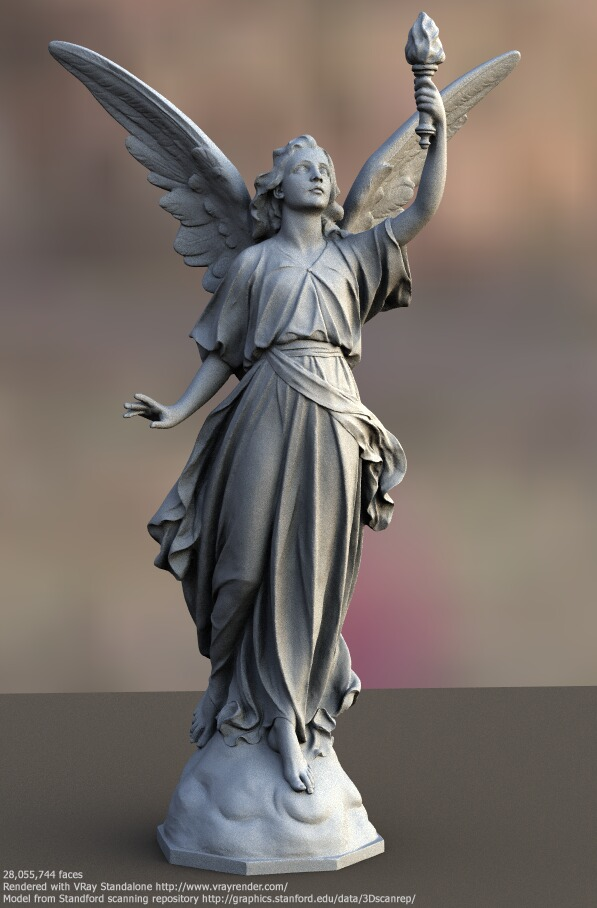
\includegraphics[scale=0.27]{angel_lucy}
\caption{Nube de puntos con reconstrucción de superficie representando una figura de un ángel.}\label{fig:angel_lucy}
\end{figure}

No solamente se pueden representar objetos mediante nubes de puntos sino entornos abiertos o interiores. Johannes Schauer y Andreas Nüchter de la universidad de Würzburg, Alemania, tomaron una nube de puntos del mercado en la ciudad de Würzburg tal y como se ve en la figura \ref{fig:wue_city}
El escaner utilizado en el este caso es el Riegl VZ-400 y con un total de 6 escaneos se han conseguido 86585411 puntos conteniendo cada uno de ellos información sobre la reflectancia de la luz del sensor lo que se aprecia con puntos de diferente claridad ya que no hay información sobre color. Obviamente, un entorno exterior contiene mucha más información que un simple objeto por lo que esta nube de puntos tiene un peso de 5117MB descomprimida.

Cabe destacar que el sensor utilizado es bastante más potente que el anteriormente mencionado y tiene un precio de unos 80000 dólares.

%http://www.riegl.com/uploads/tx_pxpriegldownloads/10_DataSheet_VZ-400_2017-06-14.pdf
%https://www.ebay.pl/itm/Riegl-VZ-400-3D-Terrestrial-Laser-Scanner-/331738609542

\begin{figure}
\centering
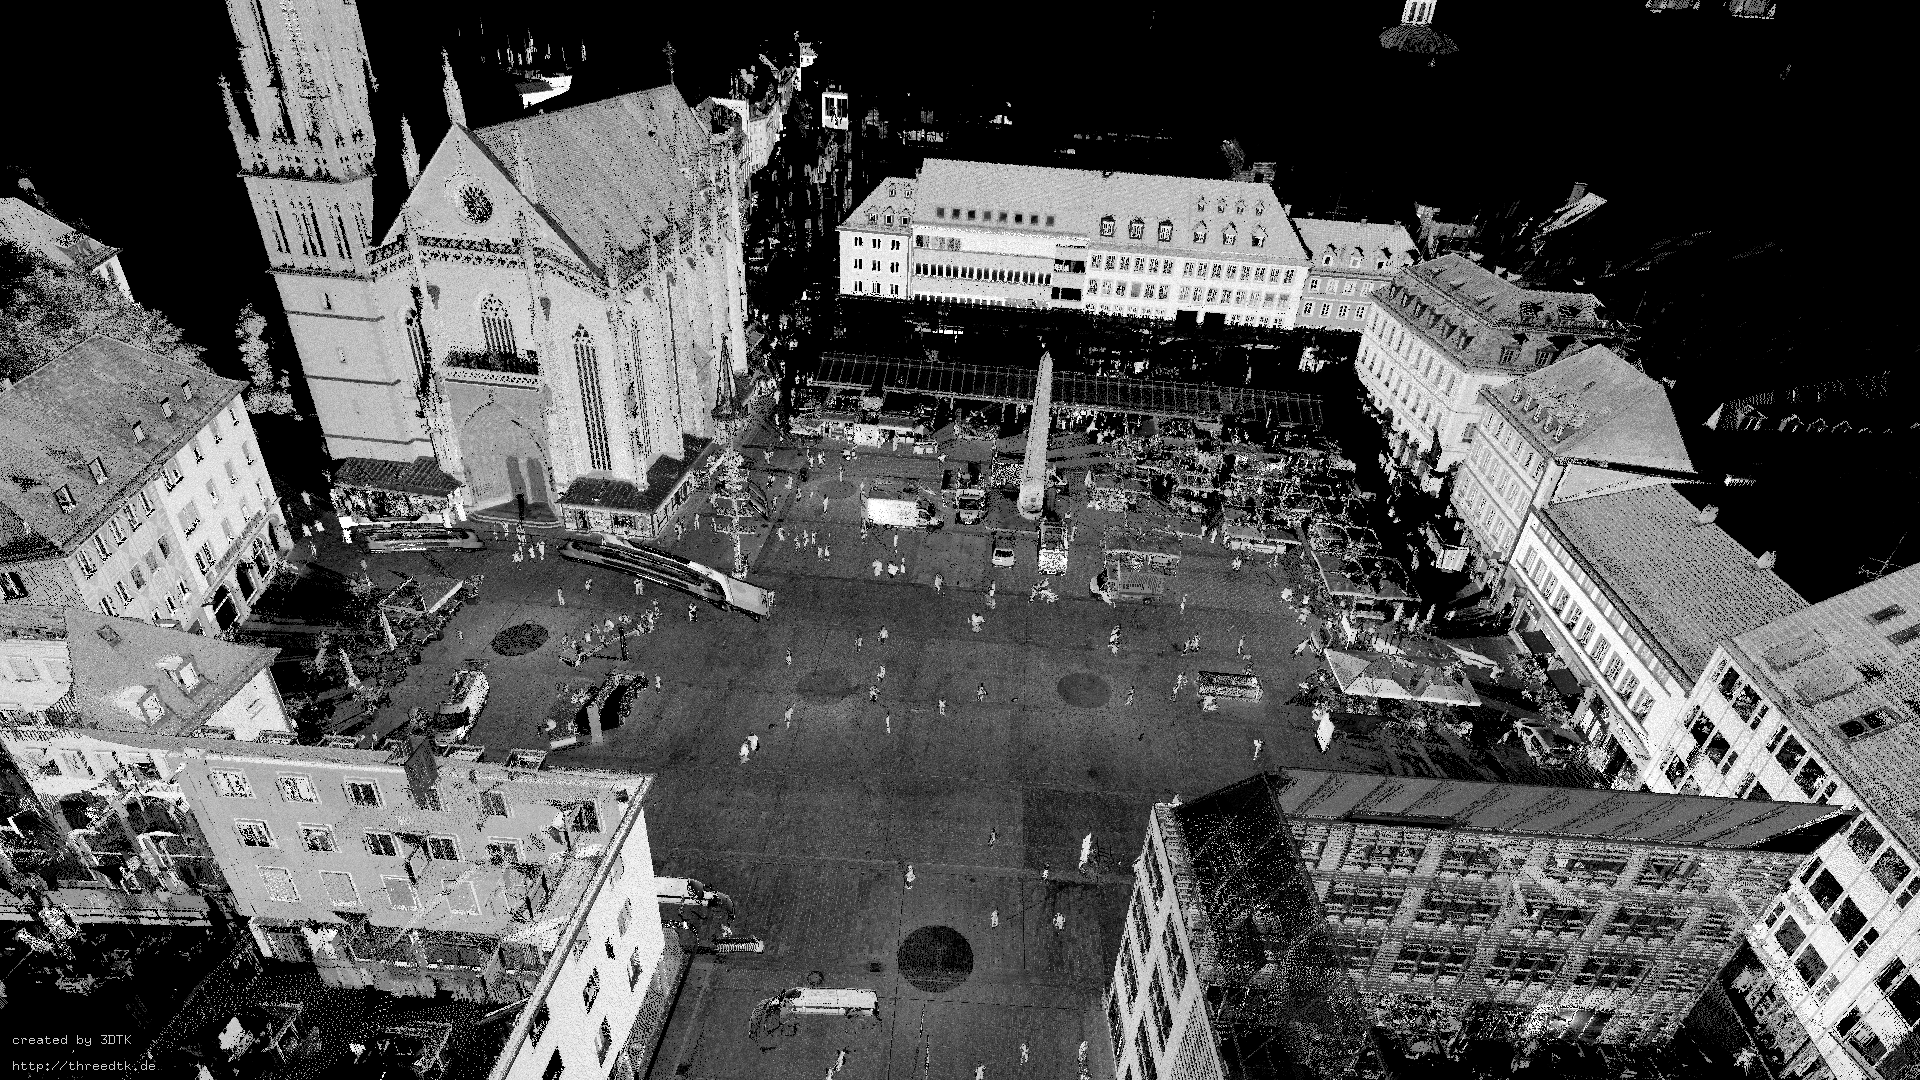
\includegraphics[scale=0.17]{wue_city2}
\caption{Nube de puntos con información de reflectancia de la luz que representa un mercado en Würzburg, Alemania.}\label{fig:wue_city}
\end{figure}

Por último, Dorit Borrmann obtuvo una nube de puntos que representa el interior del laboratorio de automática en la universidad de Jacobs, Bremen. Se pueden apreciar diferentes tipos de puntos para cada sección de la imagen ya que el sensor láser Riegl VZ-400 se encarga de representar información térmica y de profundidad mientras que las cámaras Optris PI IR y Logitech QuickCam 9000 Pro muestran información relacionada con el color.

\begin{figure}
\centering
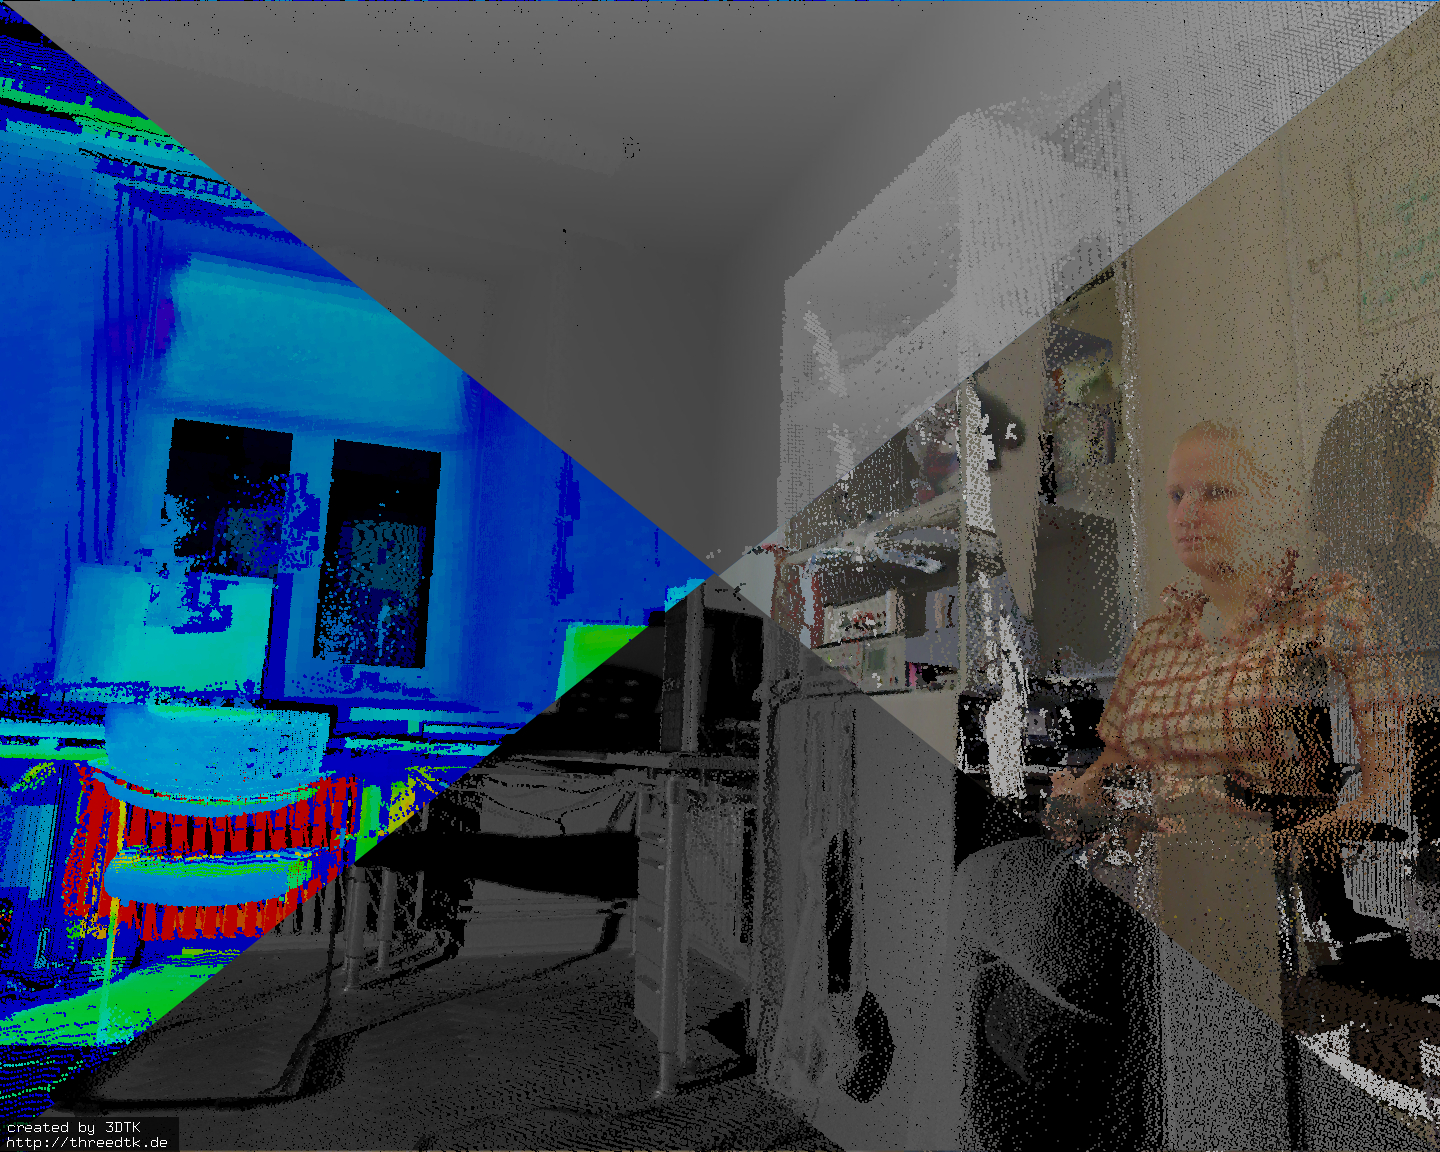
\includegraphics[scale=0.17]{joinedmodel}
\caption{Unión de cuatro nubes de puntos con información térmica, de color y reflectancia de la luz representando un entorno cerrado.}\label{fig:joined_model}
\end{figure}

Se hicieron un total de 9 escaneos en 40º cada uno lo que permite disponer de una imagen en 360º (la imagen mostrada es uno de los escaneos)

Se han visto varios ejemplos que muestran la potencia del concepto de nube de puntos y es ahora el momento de conocer cómo se ha transformado una porción de la realidad en un conjunto de puntos que la representan.
\section{Adquisición de información: Sensores y evolución}

La adquisición y almacenamiento de información es el primer paso para comenzar a trabajar con una nube de puntos. A pesar de tratarse de información relativamente sencilla como coordenadas respecto a un sistema de referencia, color y reflectividad, hay que tomar dicha información para miles o incluso millones de puntos tal y como se ha visto en ejemplos mostrados anteriormente como en el caso del ángel Lucy (figura ). Por lo tanto, el factor limitante del sensor en cuestión radica en cuánta y cuan variada información es capaz de percibir y almacenar.

En los últimos veinte años, se han hecho grandes progresos en lo que a sensores se refiere ya que actualmente se usan de sofisticadas cámaras y escaneres láser y se han dejado atrás los sensores basados en sonar o infrarrojos los cuales proporcionan a penas unos bytes de información sobre el entorno u objeto que tratan de representar.

\subsection{Sensores láser}
Centrándose en los sensores láser, la adquisición de información cobra sentido cuando se estudia el comportamiento de los rayos de luz ya sea visible o infrarroja, por ejemplo. Para poder llevar a cabo el escaneo de objetos tridimensionales así como entornos, se usa el escaneo laser o también conocido como lidar (light detection and ranging pero originalmente se conocía por la union de light and radar), 
procedimiento que se originó a principios de la década de los sesenta tras la invención del láser y que permite medir distancias a un objetivo iluminándolo con pulsos láser.


Pero ¿Cómo se pueden medir distancias utilizando luz? el concepto entorno al que el escaner laser gira es el tiempo de vuelo. Esto quiere decir que se utiliza un dispositivo (range finder) capaz de medir con precisión el tiempo que transcurre desde que se emite un pulso de luz hasta que vuelve otra vez al mismo tras rebotar sobre el objeto que desea detectarse. Considerando entonces que la velocidad de la luz es una constante conocida, c, la distancia del escaner a un punto en concreto donde rebota un determinado pulso de luz puede determinarse como:

\begin{equation}
d = \frac{c*t}{2}
\end{equation}


Nótese que $c*t$ es la distancia que hay entre el escaner y el objeto duplicada ya que $t$ es el tiempo total desde la emisión del pulso de luz hasta la recepción. Por tanto, tomando la mitad del tiempo total de vuelo se obtiene la medida deseada que es la distancia del escaner al objeto.

\begin{figure}
\centering
\minipage{0.6\textwidth}
  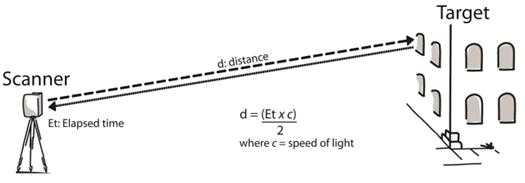
\includegraphics[width=\linewidth]{lidar_explanation}
  \caption{Ejemplo ilustrativo de medición de distancia de un sensor lidar a un edificio}\label{fig:lidar explanation}
\endminipage\hfill

\end{figure}

Para cada pulso de luz emitido se detecta un punto en concreto lo que hace pensar que para poder crear nubes con millones de puntos la velocidad de generación de los pulsos ha de ser elevada. En el caso de lidar se pueden emitir hasta 150000 pulsos en un segundo.

De este modo, al ser capaz de medir la distancia que hay desde el punto de emisión de los rayos de luz hasta la superficie en la que rebotan, el sensor puede detectar rápidamente formas definidas de objetos, edificios o paisajes considerando en conjunto de puntos detectados tal y como se ha mostrado en ejemplos del apartado \ref{section:nubes_ejemplo}

\subsubsection{Características y control de la luz utilizada por el sensor}
El componente esencial en un sistema lidar es el rayo de luz que permite hacer las mediciones. Los láseres con que tienen entre 600 y 1000 nm de longitud de onda no suelen usarse para fines científicos y debido a que pueden ser fácilmente absorbidos por el ojo deben tener potencia limitada para que su uso sea seguro.
Por otra parte, los láseres con 1550nm de longitud de onda son una buena alternativa a los anteriores ya que no son focalizados por el ojo lo que los hace seguros con potencias mucho más elevadas. Este tipo de longitudes de onda se utiliza para aplicaciones a largo alcance que no requieren elevada precisión. 

Por lo general, hay dos tipos de lidar:
método coherente e incoherente o también conocido como detección de energía directa.
El método incoherente mide cambios en la amplitud de la onda emitida pues al rebotar e interactuar con el ambiente su nivel de energía varía.
El método coherente es más apropiado para medir diferencias en la frecuencia de la onda y utiliza modulación en fase y/o frecuencia de la misma lo que le permite operar a potencias mucho más bajas a costa de utilizar un equipamiento mucho más complejo.


En ambos modelos se pueden usar dos tipos diferentes de pulsos: micropulsos y sistemas de alta energía.
los micropulsos surgen de la elevada capacidad computacional de las computadoras actuales. Esto deriva en un láser de baja potencia (del orden del microjulio) que es clasificado como seguro al ojo permitiéndose su uso bajo escasas medidas de precaución 

Por otra parte, los sistemas de alta energía, requieren medidas de seguridad más estrictas y se usan principalmente para fines de investigación atmosférica pues permite tomar medidas como la altura, número de capas y densidad de las nubes, propiedades de las partículas en las nubes, temperatura, presión, concentración de gases, o humedad.

En cuanto al control del láser, en la mayoría de los escaneres, la dirección de emisión del rayo de luz es constante por lo que para poder apuntar el haz hacia la dirección deseada se hace uso de espejos. Esto implica lanzar el láser contra un espejo y controlar éste con diferentes movimientos de rotación; en un eje para un movimiento unidimensional (un grado de libertad) o en dos ejes para un alcance espacial total quedando fija la posición del foco emisor(dos grados de libertad)

\begin{figure}[!htb]
\minipage{0.32\textwidth}
  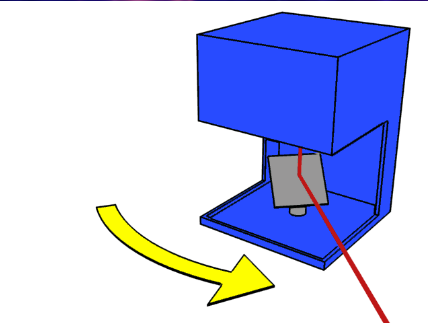
\includegraphics[width=\linewidth]{sensor_laser_espejo}
  \caption{Láser proyectado contra un espejo con un grado de libertad}\label{fig:sensor laser completo - espejo}
\endminipage\hfill
\minipage{0.32\textwidth}
  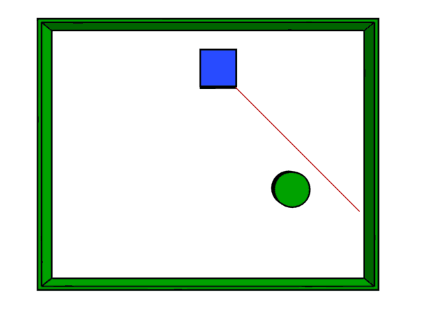
\includegraphics[width=\linewidth]{sensor_laser_vista_tope}
  \caption{Vista superior del sensor y las superficies que obstaculizan el haz de luz: objeto y recinto en el que se encuentra}\label{fig:sensor laser completo - vista tope}
\endminipage\hfill
\minipage{0.32\textwidth}
  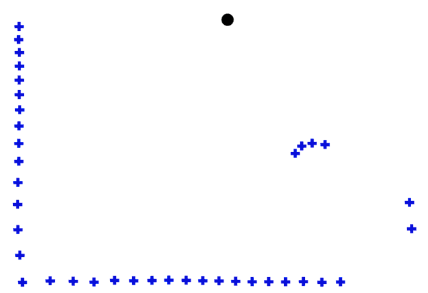
\includegraphics[width=\linewidth]{sensor_laser_resultado}
  \caption{Conjunto de puntos obtenidos tras el esacaneo pertenecientes al objeto en el interior del recinto y las limitaciones espaciales del mismo.}\label{fig:sensor laser completo - resultado}
\endminipage
\end{figure}

Una alternativa para controlar el rayo láser en dos dimensiones incumbe el uso de dos espejos montados en ejes ortogonales y entonces hacer movimientos de rotación entorno a un eje para cada uno de los espejos.

\begin{figure}
\minipage{0.45\textwidth}
  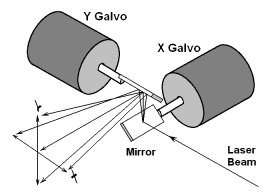
\includegraphics[width=\linewidth]{sensor_dos_espejos}
  \caption{Uso de dos espejos con un grado de libertad en cada uno y accionados con galvanómetros}\label{fig:sensor dos espejos}
\endminipage\hfill
\minipage{0.45\textwidth}
  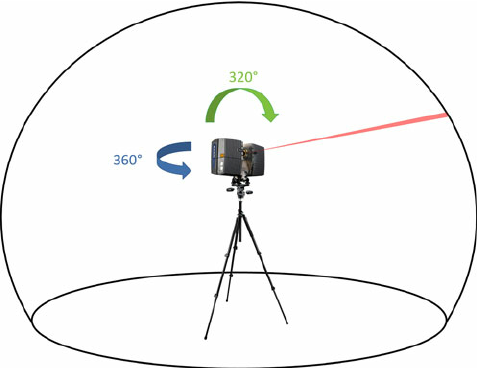
\includegraphics[width=\linewidth]{movimiento_lidar_2D}
  \caption{Sensor lidar con dos grados de libertad.}\label{fig:movimiento lidar 2D}
\endminipage\hfill

\end{figure}


para sistemas más sofisticados todavía, se requiere el posicionamiento espacial del foco emisor de rayos lo cual se consigue con un sistema de lentes servo controladas conocido como focus shifter o z-shifter

La forma más común de mover los espejos es mediante el uso de un motor eléctrico o un galvanómetro para el más sencillo de los casos. Se pueden utilizar también actuadores piezoeléctricos o magnetorresistivos para una mayor velocidad angular pero a costa de menores ángulos máximos de desplazamiento

\subsubsection{Ventajas y desventajas de lidar}

Retomando la idea de que la velocidad de la luz es una constante, la única variable en el cálculo de la distancia es el tiempo de vuelo. Téngase por ejemplo una distancia de 30cm desde el sensor hasta el objeto que desea capturarse. Esto implica que la resolución del reloj integrado en el sensor ha de ser cuanto menos elevada:

\begin{equation}
\frac{0.3m}{3*10^{8}\frac{m}{s}} = 1ns =0,000000001s
\end{equation}

Se ha desvelado de esta forma una desventaja del concepto de tiempo de vuelo, se necesita equipamiento muy preciso y fiable lo que se traduce en complejidad y elevadas inversiones económicas.

Pero dando la vuelta a esta desventaja, es decir, cuando se trata de escanear objetos en la lejanía como puede ser un edificio o paisaje, la resolución requerida por parte del reloj se reduce dando así medidas más fiables. Además, considerando de nuevo la velocidad de la luz como una constante, no importa la distancia a la que se encuentre el objeto salvo por cuestiones de difracción y absorción del pulso de luz en el ambiente, por ejemplo, por la presencia de humedad.

Por lo tanto, el método lidar combina precisión y versatilidad ya que puede valerse de luz visible, infrarroja o ultravioleta para lanzarla contra objetivos de diversos tipos de materiales como metal, cerámica, aerosoles, terreno (rocas y tierra) e incluso se puede llegar al nivel molecular. 
 
Sin embargo no se realiza un único escaneo ya que el propio concepto implica que el objeto bloquea los rayos de luz por lo que la cara frontal, de la que sí se obtiene información, impide a la luz llegar a la cara posterior. El factor clave es entonces el hecho de que estos rayos de luz puedan llegar a toda la superficie del objeto que se quiere analizar, es decir, accesibilidad física del sensor.
De este modo, independientemente del sensor o método que se utilice, es imposible recolectar
información sobre superficies no visibles o lo que es lo mismo, con un solo escaneo.

Este efecto puede apreciarse en la figura \ref{fig:botes} donde falta información en el seno de la nube de puntos en forma de tres áreas en las que no hay ningún punto pues son la "sombra" de los botes ante los rayos de luz del escaner.

Como consecuencia, es necesario llevar a cabo varios escaneos desde diferentes puntos de vista y
ponerlos en conjunto conociendo con precisión la posición del sensor en cada escaneo para poder llevar a cabo lo que se conoce como alineamiento de nubes de puntos, concepto que se explicará con más detalle posteriormente.


\subsubsection{Aplicaciones de lidar}

Una aplicación muy extendida del lidar es el reconocimiento de terreno. Para ello se integra el sensor en una aeronave y se capturan los puntos correspondientes al terreno sobrevolado. Esta aplicación es útil para generar modelos digitales de elevación.

Como contrapartida, hay que tener en cuenta que el sensor tiene una posición variable respecto al terreno ya que va embarcado en una aeronave. Para considerar esto en el resultado final de la nube de puntos generada, se ha de disponer de un sistema de navegación, para el posicionamiento del sensor con GPS por ejemplo, así como de una unidad de medidas inerciales (IMU inertial maesurement unit), para obtener información sobre la orientación absoluta del sensor.

 
\begin{figure}
\minipage{0.45\textwidth}
  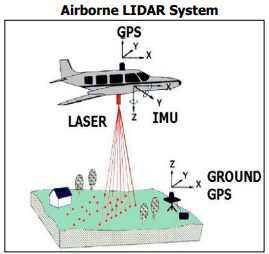
\includegraphics[width=\linewidth]{airborne_lidar}
  \caption{Esquema de utilización del método lidar en una aeroanve}\label{fig:airborne_lidar}
\endminipage\hfill
\minipage{0.45\textwidth}
  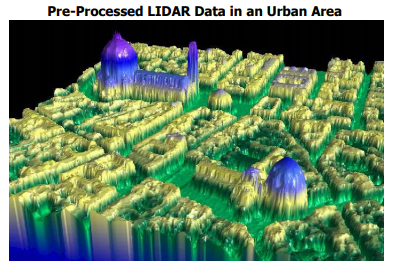
\includegraphics[width=\linewidth]{airborne_city}
  \caption{Entorno urbano recreado con el método lidar}\label{fig:airborne_city}
\endminipage\hfill

\end{figure}




%https://upload.wikimedia.org/wikipedia/commons/c/c0/LIDAR-scanned-SICK-LMS-animation.gif
%https://www.engineering.com/AdvancedManufacturing/ArticleID/12390/Quality-Basics-How-Does-3D-Laser-Scanning-Work.aspx
%https://en.wikipedia.org/wiki/Laser_scanning
%http://www.2grobotics.com/wp-content/uploads/2017/03/sonarvslaser.pdf
%http://www.lidar-uk.com/how-lidar-works/
%http://elm-chan.org/works/vlp/report_e.html
%http://www.ionix.fi/en/technologies/laser-processing/laser-marking/
%https://blog.cometlabs.io/engineer-explains-lidar-748f9ba0c404

\subsection{Alternativas a lidar}

Disponer de complejas, fiables y robustas representaciones del mundo real tiene no es tan sencillo como pueda parecer puesto que estos sensores suelen tener un precio prohibitivo para la mayoría de los interesados ya sean particulares o incluso empresas con un poder adquisitivo considerable. Véanse por ejemplo los sensores mencionados en el apartado \ref{section:nubes_ejemplo} los cuales tienen un precio de más de 70000\$

Sin embargo, la situación ha cambiado desde que han aparecido en el mercado ciertos sensores 3D como por ejemplo el sensor Kinect de la consola Xbox360 de Microsoft. Este sensor está basado en la tecnología PrimeSense y aunque puede trabajar con nubes de puntos en tiempo real e imágenes en 2D su precio no supera los 150\$. De este modo se ha producido un gran paso adelante en cuanto a los impedimentos relacionados con la adquisición, mantenimiento y delicadeza del hardware que traduce el mundo real a nubes de puntos.

%https://www.matec-conferences.org/articles/matecconf/pdf/2018/32/matecconf_smima2018_03001.pdf
%https://erget.wordpress.com/2014/04/27/producing-3d-point-clouds-with-a-stereo-camera-in-opencv/

\section{Procesamiento software de información }

Una vez registradas y almacenadas las nubes de puntos, se precisa ahora de un mecanismo para trabajar con la inmensa cantidad de información que aportan los sensores. El software existente para dicha tarea es diverso y no siempre gratuito. Como ejemplo se tiene RealityCapture o RC, un software capaz de crear modelos 3D a partir de fotografías o escaneos láser desordenados. Su alcance abarca aspectos como arte, arquitectura, escaneo completo del cuerpo humano, videojuegos, mapeado, efectos visuales y realidad virtual.

Entre sus características se encuentran cálculo de redes de polígonos, coloreado, texturizado, georreferenciación, conversión de sistema de coordenadas, suavizado y operaciones de lectura/escritura o input/output.
El software puede ejecutarse por línea de comandos o mediante un kit de desarrollo.

A pesar de que puede llegar a mezclar imágenes de cámara y escaneos láser, este software está diseñado para desarrollar bajas exigencias de hardware. 

Trabaja de forma lineal lo que significa que si las entradas se duplican también lo hará el tiempo de ejecución.

Este software está disponible solamente en inglés y sus requerimientos son su punto débil ya que necesita una máquina de 64 bits con al menos 8 GB de RAM y una versión de windows superior a windows 7. Además, se puede disponer de forma opcional de una GPU nVidia CUDA de al menos 1GB de RAM si se desea crear redes texturizadas.

Cada licencia está limitada a 32 núcleos de procesador y 3 tarjetas gráficas. Para configuraciones superiores, se pueden adquirir más licencias. Se recomienda una computadora con un procesador de 4 núcleos, 16GB de RAM y una CUDA 386.



Existe más software semejante al descrito y la inmensa mayoría tiene limitaciones de licencias o de hardware demasiado potente, y por lo tanto de un valor económico elevado, para un usuario particular. Pero entre todos ellos destaca PCL, siglas que en inglés se refieren a Point Cloud Library, es decir, librería de nubes de puntos. Es una librería única, de gran escala y un proyecto abierto a la comunidad para procesamiento de imágenes y nubes de puntos tanto en 2D como en 3D. Es más, PCL se somete a os términos de la licencia BSD (Berkelay Software Distribution) lo que implica que es de uso libre tanto para fines comerciales como de investigación. 

\begin{figure}
\centering
\minipage{0.45\textwidth}
  
\includegraphics[width=\linewidth]{pcl_logo}
  \caption{Logo de PCL}\label{fig:pcl logo}
\endminipage\hfill
\end{figure}

PCL dispone de multitud de herramientas para el procesamiento de nubes de puntos y dado que es una librería sometida a constante crecimiento y modificaciones, tener las herramientas debidamente organizadas y estructuradas es de vital importancia. Es por esto por lo que PCL tiene una organización en forma de librerías modulares, es decir, el conjunto de herramientas se clasifica según su utilidad.

Uno de los módulos más importantes es el que se encarga de la lectura y escritura de nubes de puntos, es decir, el módulo IO del inglés input/output que se traduce como entrada/salida. Es por tanto esta librería capaz de interpretar la información otorgada por diferentes tipos de sensores así como de generar archivos que contienen nubes de puntos manipuladas por el resto de módulos.
Existen varios tipos de formatos bajo los que almacenar una nube puntos.

PCL ha creado el formato PCD, del inglés Point Cloud Data, es decir datos de nube de puntos. No se trata de un formato revolucionario sino más bien de una forma de complementar a los ya existentes que debido a los propósitos para los que se han creado u otras razones, no soportan algunas de las características relacionas con al procesamiento de nubes de puntos de n dimensiones. Además sufren de deficiencias en ciertos campos de computación debido a que fueron creados para fines diferentes, en diferentes épocas y en ocasiones mucho antes de la invención de los sensores y algoritmos hoy presentes.

Por lo tanto, el formato PCD no es único ni trata de reemplazar a los que ya están presentes creados por comunidades de computación gráfica y geométrica que en concreto sirven para describir polígonos arbitrarios y nubes de puntos obtenidas con escáneres láser. Por ejemplo se tienen formatos como los siguientes:


PLY - Formato de ficheros para polígonos creado por Turk et al de la universidad de Stanford
STL - Un formato nativo para software CAD de estereolitografía creado por 3D systems 
OBJ - Un software de definición geométrica creado por Wavefront Technologies 
X3D - Un formato basado en la norma ISO de XML para la representación de gráficos en 3d para computadoras 

Puesto que a partir de ahora se va a utilizar el formato PCD, se va a explicar con mayor profundidad cada una de sus partes.

Un fichero PCD dispone de dos partes diferenciadas, encabezamiento y los puntos como tal.

El encabezamiento se encarga de identificar y declarar las propiedades de la nube de puntos almacenados en el fichero y debe estar codificado en ASCII lo que implica que cada entrada en este formato está delimitada de las demás usando saltos de línea.

Las características especificadas en el encabezamiento son las siguientes:

\begin{itemize}
\item VERSION:
Este campo especifica la versión del formato PCD

\item FIELDS
Traducido como "campos" indica el nombre de cada dimensión o campo existente en la nube de puntos como por ejemplo color, coordenadas XYZ o normales a la superficie.

\item SIZE 
Este campo indica el tamaño en bytes y en el mismo orden de cada campo declarado por FIELDS 

\item TYPE
Representa el tipo de dato de cada campo con un carácter. 
I: Tipos con signo como int8 que equivale a un char, int16 que equivale a un short y int32 que equivale a un int
U: Tipos sin signo como uint8, uint16 y uint32, los tipos análogos al caso anterior pero sin signo
F: Representa todos los tipos flotantes

\item COUNT 
Indica cuántos elementos tiene cada campo previamente declarado en FIELDS. Por defecto toma el valor de 1.

\item WIDTH
Representa el ancho de la nube de puntos teniendo este concepto dos significados para lo cual hay que entender cómo se puede interpretar una nube de puntos. Por una parte, las nubes de puntos desorganizadas pueden verse como un vector de n elementos donde n es el ancho de la nube de puntos, es decir, se trata de una matriz de una fila y n columnas donde n es el ancho. Por otra parte, se puede definir de manera matricial con m filas y n columnas siendo ahora m el número de puntos presentes en cada columna y lo que define una nube de puntos organizada.

\item HEIGHT
No es nada más que el número de filas de la nube de puntos en su representación matricial explicada en el apartado anterior o bien el numero total de puntos de una nube representada como una matriz de m filas y una columna siendo en este caso m el campo tratado en este apartado.

\item VIEWPOINT
Especifica la posición del punto de vista desde el que el sensor adquirió la nube de puntos. Se indica como una traslación tx, ty, tz así como con un cuaternio qw, qx, qy, qz con un valor por defecto de 0 0 0 1 0 0 0 respectivamente.

\item POINTS
Indica el número total de puntos en la nube. Puesto que se trata de información redundante dados los campos previamente descritos, se espera que éste sea eliminado en un futuro.

\item DATA
Es el tipo de dato con el que se ha generado el fichero PCD siendo dos formatos los soportados, ascii y binary. El formato ascii obliga a que cada punto se escriba en una nueva línea, mientras que en el formato binary, la información presente en el fichero es una copia en memoria de la nube de puntos como vector de forma que se incrementa la velocidad de lectura y escritura
\end{itemize}

Queda el encabezamiento entonces con la siguiente estructura:

VERSION\\
FIELDS\\
SIZE\\
TYPE\\
COUNT\\
WIDTH\\
HEIGHT\\
VIEWPOINT\\
POINTS\\
DATA\\

Como se ha mencionado previamente, cada punto se introduce después del encabezado en una línea nueva indicando, separados por espacios, el valor de cada campo. Como ejemplo de nube de puntos en formato PCD se tiene lo siguiente:

VERSION .7\\
FIELDS x y z rgb\\
SIZE 4 4 4 4\\
TYPE F F F F\\
COUNT 1 1 1 1\\
WIDTH 213\\
HEIGHT 1\\
VIEWPOINT 0 0 0 1 0 0 0\\
POINTS 5\\
DATA ascii\\
0.93773 0.33763 0 4.2108e+06\\
0.90805 0.35641 0 4.2108e+06\\
0.81915 0.32 0 4.2108e+06\\
0.97192 0.278 0 4.2108e+06\\
0.944 0.29474 0 4.2108e+06\\

A parte del módulo básico de lectura y escritura, PCL dispone de herramientas de filtrado por ejemplo. Esto se refiere a la criba o eliminación de puntos no deseados y los cuales representan ruido, por ejemplo.

Se muestra un ejemplo en la siguiente figura en la que se aprecia que, debido a errores de medida, ciertas nubes de puntos presentan un elevado número de puntos que representan sombras. Esto complica las operaciones de estimación de propiedades locales. Algunos de estos puntos pueden eliminarse llevando a cabo un análisis en la vecindad de cada punto y eliminar aquellos vecinos que no cumplen ciertos requisitos. Por ejemplo, se puede tomar como criterio la distancia de cada vecino al punto estudiado, es decir, se toma la media de las distancias de todos los vecinos al punto estudiado y si la desviación a esa media de un vecino supera cierto valor entonces es eliminado.
\begin{figure}
\centering
\minipage{0.75\textwidth}
  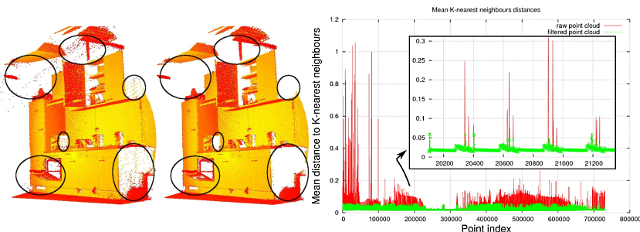
\includegraphics[width=\linewidth]{pcl_filter}
  \caption{Filtrado de ruido mediante el módulo filter de PCL}\label{fig:pcl_filter}
\endminipage\hfill
\end{figure}

Explicar modulos filter, viewer y keypoints

\section{objetivos}
Generar un programa capaz de obtener keypoints a partir de una nube de puntos
Croscompilar usando las herramientas de xilinx 
Enviar ejecutable a la placa y ejecutar el programa
(optimización)

%http://pointclouds.org/


\section{Descripción de herramientas}
\subsection{Herramientas hardware}
\subsection{Herramientas software}




